%%%%%%%%%%%%%%%%%%%%%%%%%%%%%%%%%%%%%%%%%%%%%%%%%%%%%%%%%%%%%%%%%%%%%%%%%%%
%% This file is part of the book
%%
%% Algorithmic Graph Theory
%% http://code.google.com/p/graph-theory-algorithms-book/
%%
%% Copyright (C) 2009, 2010, 2011 Minh Van Nguyen <nguyenminh2@gmail.com>
%%
%% See the file COPYING for copying conditions.
%%%%%%%%%%%%%%%%%%%%%%%%%%%%%%%%%%%%%%%%%%%%%%%%%%%%%%%%%%%%%%%%%%%%%%%%%%%

\subfigure[]{
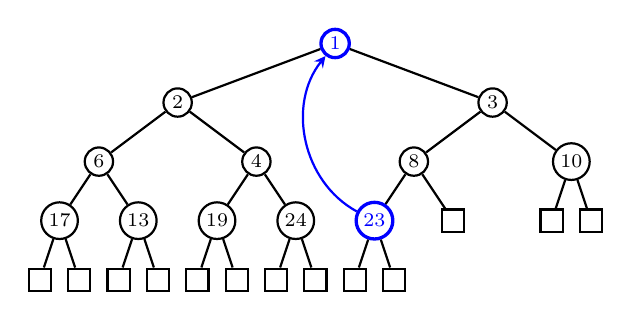
\begin{tikzpicture}
[-,thick,%
  every node/.style={shape=circle,inner sep=1.5pt,draw,thick},%
  scale=0.5]
\scriptsize
\node[blue,very thick] (1) {$1$}
  [sibling distance=8cm]
  child {node {$2$}
    [sibling distance=4cm]
    child {node {$6$}
      [sibling distance=2cm]
      child {node {$17$}
        [sibling distance=1cm]
        child {node[rectangle,inner sep=4pt,draw,thick] {}}
        child {node[rectangle,inner sep=4pt,draw,thick] {}}
      }
      child {node {$13$}
        [sibling distance=1cm]
        child {node[rectangle,inner sep=4pt,draw,thick] {}}
        child {node[rectangle,inner sep=4pt,draw,thick] {}}
      }
    }
    child {node {$4$}
      [sibling distance=2cm]
      child {node {$19$}
        [sibling distance=1cm]
        child {node[rectangle,inner sep=4pt,draw,thick] {}}
        child {node[rectangle,inner sep=4pt,draw,thick] {}}
      }
      child {node {$24$}
        [sibling distance=1cm]
        child {node[rectangle,inner sep=4pt,draw,thick] {}}
        child {node[rectangle,inner sep=4pt,draw,thick] {}}
      }
    }
  }
  child {node {$3$}
    [sibling distance=4cm]
    child {node {$8$}
      [sibling distance=2cm]
      child {node[blue,very thick] (23) {$23$}
        [sibling distance=1cm]
        child {node[rectangle,inner sep=4pt,draw,thick] {}}
        child {node[rectangle,inner sep=4pt,draw,thick] {}}
      }
      child {node[rectangle,inner sep=4pt,draw,thick] {}}
    }
    child {node {$10$}
      [sibling distance=1cm]
      child {node[rectangle,inner sep=4pt,draw,thick] {}}
      child {node[rectangle,inner sep=4pt,draw,thick] {}}
    }
  };
\path
(23) edge[->,>=stealth,thick,bend left=50,blue] (1);
\end{tikzpicture}
}
%%
%%
\quad
\subfigure[]{
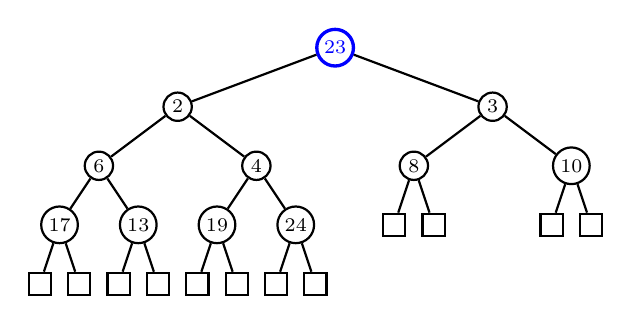
\begin{tikzpicture}
[-,thick,%
  every node/.style={shape=circle,inner sep=1.5pt,draw,thick},%
  scale=0.5]
\scriptsize
\node[blue,very thick] {$23$}
  [sibling distance=8cm]
  child {node {$2$}
    [sibling distance=4cm]
    child {node {$6$}
      [sibling distance=2cm]
      child {node {$17$}
        [sibling distance=1cm]
        child {node[rectangle,inner sep=4pt,draw,thick] {}}
        child {node[rectangle,inner sep=4pt,draw,thick] {}}
      }
      child {node {$13$}
        [sibling distance=1cm]
        child {node[rectangle,inner sep=4pt,draw,thick] {}}
        child {node[rectangle,inner sep=4pt,draw,thick] {}}
      }
    }
    child {node {$4$}
      [sibling distance=2cm]
      child {node {$19$}
        [sibling distance=1cm]
        child {node[rectangle,inner sep=4pt,draw,thick] {}}
        child {node[rectangle,inner sep=4pt,draw,thick] {}}
      }
      child {node {$24$}
        [sibling distance=1cm]
        child {node[rectangle,inner sep=4pt,draw,thick] {}}
        child {node[rectangle,inner sep=4pt,draw,thick] {}}
      }
    }
  }
  child {node {$3$}
    [sibling distance=4cm]
    child {node {$8$}
      [sibling distance=1cm]
      child {node[rectangle,inner sep=4pt,draw,thick] {}}
      child {node[rectangle,inner sep=4pt,draw,thick] {}}
    }
    child {node {$10$}
      [sibling distance=1cm]
      child {node[rectangle,inner sep=4pt,draw,thick] {}}
      child {node[rectangle,inner sep=4pt,draw,thick] {}}
    }
  };
\end{tikzpicture}
}
%%
%%
\subfigure[]{
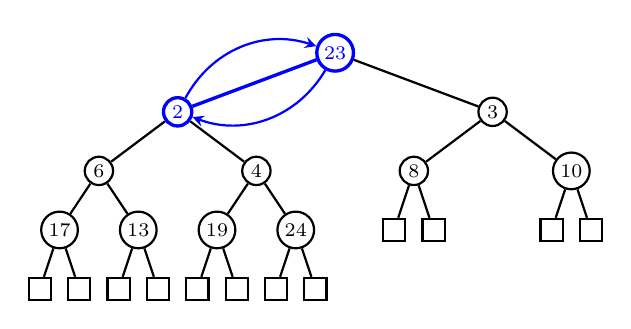
\begin{tikzpicture}
[-,thick,%
  every node/.style={shape=circle,inner sep=1.5pt,draw,thick},%
  scale=0.5]
\scriptsize
\node[blue,very thick] (23) {$23$}
  [sibling distance=8cm]
  child[blue,very thick] {node[blue,very thick] (2) {$2$}
    [sibling distance=4cm]
    child[black,thick] {node {$6$}
      [sibling distance=2cm]
      child {node {$17$}
        [sibling distance=1cm]
        child {node[rectangle,inner sep=4pt,draw,thick] {}}
        child {node[rectangle,inner sep=4pt,draw,thick] {}}
      }
      child {node {$13$}
        [sibling distance=1cm]
        child {node[rectangle,inner sep=4pt,draw,thick] {}}
        child {node[rectangle,inner sep=4pt,draw,thick] {}}
      }
    }
    child[black,thick] {node {$4$}
      [sibling distance=2cm]
      child {node {$19$}
        [sibling distance=1cm]
        child {node[rectangle,inner sep=4pt,draw,thick] {}}
        child {node[rectangle,inner sep=4pt,draw,thick] {}}
      }
      child {node {$24$}
        [sibling distance=1cm]
        child {node[rectangle,inner sep=4pt,draw,thick] {}}
        child {node[rectangle,inner sep=4pt,draw,thick] {}}
      }
    }
  }
  child {node {$3$}
    [sibling distance=4cm]
    child {node {$8$}
      [sibling distance=1cm]
      child {node[rectangle,inner sep=4pt,draw,thick] {}}
      child {node[rectangle,inner sep=4pt,draw,thick] {}}
    }
    child {node {$10$}
      [sibling distance=1cm]
      child {node[rectangle,inner sep=4pt,draw,thick] {}}
      child {node[rectangle,inner sep=4pt,draw,thick] {}}
    }
  };
\path
(2) edge[->,>=stealth,thick,bend left=40,blue] (23)
(23) edge[->,>=stealth,thick,bend left=40,blue] (2);
\end{tikzpicture}
}
%%
%%
\quad
\subfigure[]{
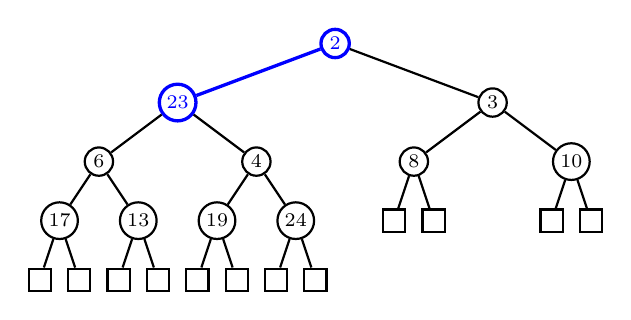
\begin{tikzpicture}
[-,thick,%
  every node/.style={shape=circle,inner sep=1.5pt,draw,thick},%
  scale=0.5]
\scriptsize
\node[blue,very thick] {$2$}
  [sibling distance=8cm]
  child[blue,very thick] {node[blue,very thick] {$23$}
    [sibling distance=4cm]
    child[black,thick] {node {$6$}
      [sibling distance=2cm]
      child {node {$17$}
        [sibling distance=1cm]
        child {node[rectangle,inner sep=4pt,draw,thick] {}}
        child {node[rectangle,inner sep=4pt,draw,thick] {}}
      }
      child {node {$13$}
        [sibling distance=1cm]
        child {node[rectangle,inner sep=4pt,draw,thick] {}}
        child {node[rectangle,inner sep=4pt,draw,thick] {}}
      }
    }
    child[black,thick] {node {$4$}
      [sibling distance=2cm]
      child {node {$19$}
        [sibling distance=1cm]
        child {node[rectangle,inner sep=4pt,draw,thick] {}}
        child {node[rectangle,inner sep=4pt,draw,thick] {}}
      }
      child {node {$24$}
        [sibling distance=1cm]
        child {node[rectangle,inner sep=4pt,draw,thick] {}}
        child {node[rectangle,inner sep=4pt,draw,thick] {}}
      }
    }
  }
  child {node {$3$}
    [sibling distance=4cm]
    child {node {$8$}
      [sibling distance=1cm]
      child {node[rectangle,inner sep=4pt,draw,thick] {}}
      child {node[rectangle,inner sep=4pt,draw,thick] {}}
    }
    child {node {$10$}
      [sibling distance=1cm]
      child {node[rectangle,inner sep=4pt,draw,thick] {}}
      child {node[rectangle,inner sep=4pt,draw,thick] {}}
    }
  };
\end{tikzpicture}
}
%%
%%
\subfigure[]{
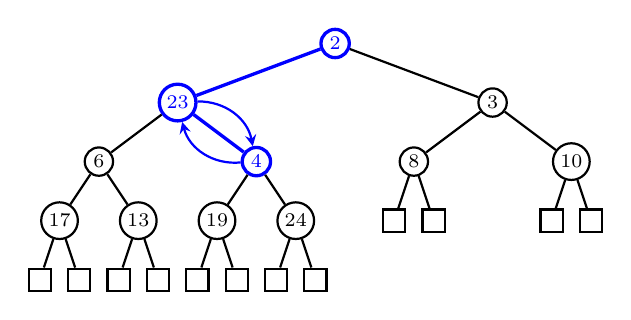
\begin{tikzpicture}
[-,thick,%
  every node/.style={shape=circle,inner sep=1.5pt,draw,thick},%
  scale=0.5]
\scriptsize
\node[blue,very thick] {$2$}
  [sibling distance=8cm]
  child[blue,very thick] {node[blue,very thick] (23) {$23$}
    [sibling distance=4cm]
    child[black,thick] {node {$6$}
      [sibling distance=2cm]
      child {node {$17$}
        [sibling distance=1cm]
        child {node[rectangle,inner sep=4pt,draw,thick] {}}
        child {node[rectangle,inner sep=4pt,draw,thick] {}}
      }
      child {node {$13$}
        [sibling distance=1cm]
        child {node[rectangle,inner sep=4pt,draw,thick] {}}
        child {node[rectangle,inner sep=4pt,draw,thick] {}}
      }
    }
    child[blue,very thick] {node[blue,very thick] (4) {$4$}
      [sibling distance=2cm]
      child[black,thick] {node {$19$}
        [sibling distance=1cm]
        child {node[rectangle,inner sep=4pt,draw,thick] {}}
        child {node[rectangle,inner sep=4pt,draw,thick] {}}
      }
      child[black,thick] {node {$24$}
        [sibling distance=1cm]
        child {node[rectangle,inner sep=4pt,draw,thick] {}}
        child {node[rectangle,inner sep=4pt,draw,thick] {}}
      }
    }
  }
  child {node {$3$}
    [sibling distance=4cm]
    child {node {$8$}
      [sibling distance=1cm]
      child {node[rectangle,inner sep=4pt,draw,thick] {}}
      child {node[rectangle,inner sep=4pt,draw,thick] {}}
    }
    child {node {$10$}
      [sibling distance=1cm]
      child {node[rectangle,inner sep=4pt,draw,thick] {}}
      child {node[rectangle,inner sep=4pt,draw,thick] {}}
    }
  };
\path
(4) edge[->,>=stealth,thick,bend left=40,blue] (23)
(23) edge[->,>=stealth,thick,bend left=40,blue] (4);
\end{tikzpicture}
}
%%
%%
\quad
\subfigure[]{
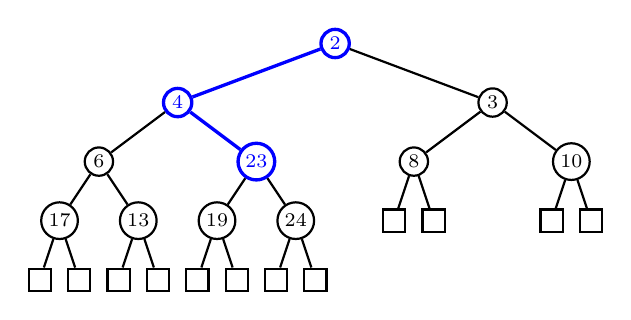
\begin{tikzpicture}
[-,thick,%
  every node/.style={shape=circle,inner sep=1.5pt,draw,thick},%
  scale=0.5]
\scriptsize
\node[blue,very thick] {$2$}
  [sibling distance=8cm]
  child[blue,very thick] {node[blue,very thick] {$4$}
    [sibling distance=4cm]
    child[black,thick] {node {$6$}
      [sibling distance=2cm]
      child {node {$17$}
        [sibling distance=1cm]
        child {node[rectangle,inner sep=4pt,draw,thick] {}}
        child {node[rectangle,inner sep=4pt,draw,thick] {}}
      }
      child {node {$13$}
        [sibling distance=1cm]
        child {node[rectangle,inner sep=4pt,draw,thick] {}}
        child {node[rectangle,inner sep=4pt,draw,thick] {}}
      }
    }
    child[blue,very thick] {node[blue,very thick] {$23$}
      [sibling distance=2cm]
      child[black,thick] {node {$19$}
        [sibling distance=1cm]
        child {node[rectangle,inner sep=4pt,draw,thick] {}}
        child {node[rectangle,inner sep=4pt,draw,thick] {}}
      }
      child[black,thick] {node {$24$}
        [sibling distance=1cm]
        child {node[rectangle,inner sep=4pt,draw,thick] {}}
        child {node[rectangle,inner sep=4pt,draw,thick] {}}
      }
    }
  }
  child {node {$3$}
    [sibling distance=4cm]
    child {node {$8$}
      [sibling distance=1cm]
      child {node[rectangle,inner sep=4pt,draw,thick] {}}
      child {node[rectangle,inner sep=4pt,draw,thick] {}}
    }
    child {node {$10$}
      [sibling distance=1cm]
      child {node[rectangle,inner sep=4pt,draw,thick] {}}
      child {node[rectangle,inner sep=4pt,draw,thick] {}}
    }
  };
\end{tikzpicture}
}
%%
%%
\subfigure[]{
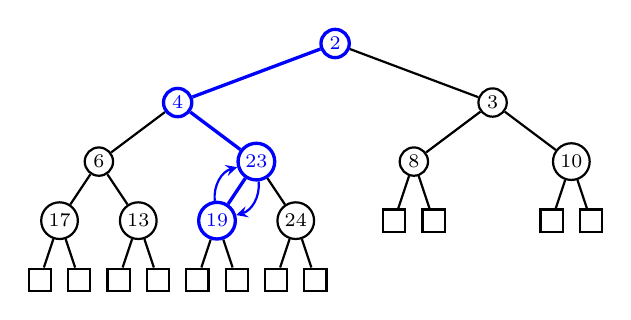
\begin{tikzpicture}
[-,thick,%
  every node/.style={shape=circle,inner sep=1.5pt,draw,thick},%
  scale=0.5]
\scriptsize
\node[blue,very thick] {$2$}
  [sibling distance=8cm]
  child[blue,very thick] {node[blue,very thick] {$4$}
    [sibling distance=4cm]
    child[black,thick] {node {$6$}
      [sibling distance=2cm]
      child {node {$17$}
        [sibling distance=1cm]
        child {node[rectangle,inner sep=4pt,draw,thick] {}}
        child {node[rectangle,inner sep=4pt,draw,thick] {}}
      }
      child {node {$13$}
        [sibling distance=1cm]
        child {node[rectangle,inner sep=4pt,draw,thick] {}}
        child {node[rectangle,inner sep=4pt,draw,thick] {}}
      }
    }
    child[blue,very thick] {node[blue,very thick] (23) {$23$}
      [sibling distance=2cm]
      child[blue,very thick] {node[blue,very thick] (19) {$19$}
        [sibling distance=1cm]
        child[black,thick] {node[rectangle,inner sep=4pt,draw,thick] {}}
        child[black,thick] {node[rectangle,inner sep=4pt,draw,thick] {}}
      }
      child[black,thick] {node {$24$}
        [sibling distance=1cm]
        child {node[rectangle,inner sep=4pt,draw,thick] {}}
        child {node[rectangle,inner sep=4pt,draw,thick] {}}
      }
    }
  }
  child {node {$3$}
    [sibling distance=4cm]
    child {node {$8$}
      [sibling distance=1cm]
      child {node[rectangle,inner sep=4pt,draw,thick] {}}
      child {node[rectangle,inner sep=4pt,draw,thick] {}}
    }
    child {node {$10$}
      [sibling distance=1cm]
      child {node[rectangle,inner sep=4pt,draw,thick] {}}
      child {node[rectangle,inner sep=4pt,draw,thick] {}}
    }
  };
\path
(19) edge[->,>=stealth,thick,bend left=40,blue] (23)
(23) edge[->,>=stealth,thick,bend left=40,blue] (19);
\end{tikzpicture}
}
%%
%%
\quad
\subfigure[]{
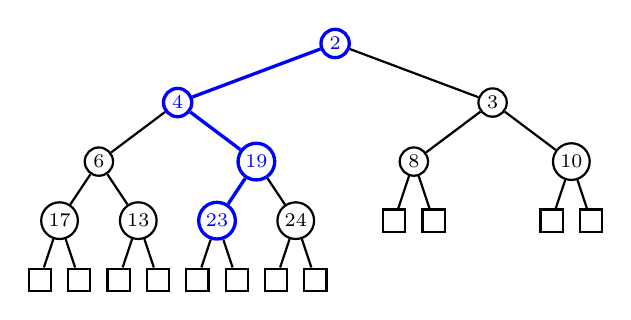
\begin{tikzpicture}
[-,thick,%
  every node/.style={shape=circle,inner sep=1.5pt,draw,thick},%
  scale=0.5]
\scriptsize
\node[blue,very thick] {$2$}
  [sibling distance=8cm]
  child[blue,very thick] {node[blue,very thick] {$4$}
    [sibling distance=4cm]
    child[black,thick] {node {$6$}
      [sibling distance=2cm]
      child {node {$17$}
        [sibling distance=1cm]
        child {node[rectangle,inner sep=4pt,draw,thick] {}}
        child {node[rectangle,inner sep=4pt,draw,thick] {}}
      }
      child {node {$13$}
        [sibling distance=1cm]
        child {node[rectangle,inner sep=4pt,draw,thick] {}}
        child {node[rectangle,inner sep=4pt,draw,thick] {}}
      }
    }
    child[blue,very thick] {node[blue,very thick] {$19$}
      [sibling distance=2cm]
      child[blue,very thick] {node[blue,very thick] {$23$}
        [sibling distance=1cm]
        child[black,thick] {node[rectangle,inner sep=4pt,draw,thick] {}}
        child[black,thick] {node[rectangle,inner sep=4pt,draw,thick] {}}
      }
      child[black,thick] {node {$24$}
        [sibling distance=1cm]
        child {node[rectangle,inner sep=4pt,draw,thick] {}}
        child {node[rectangle,inner sep=4pt,draw,thick] {}}
      }
    }
  }
  child {node {$3$}
    [sibling distance=4cm]
    child {node {$8$}
      [sibling distance=1cm]
      child {node[rectangle,inner sep=4pt,draw,thick] {}}
      child {node[rectangle,inner sep=4pt,draw,thick] {}}
    }
    child {node {$10$}
      [sibling distance=1cm]
      child {node[rectangle,inner sep=4pt,draw,thick] {}}
      child {node[rectangle,inner sep=4pt,draw,thick] {}}
    }
  };
\end{tikzpicture}
}
